\documentclass{article}
\usepackage{booktabs, graphicx}
\begin{document}
\begin{table}[h]
\centering
\begin{tabular}{| c | c | c |}\hline
Name & Type & Params \\ \hline
model & TransformerResnet & 10.5 M \\ \hline
criterion & CosineEmbeddingLoss & 0 \\ \hline
F1 score & BinaryF1Score & 0 \\ \hline
AP score & BinaryAveragePrecision & 0 \\ \hline
PR Curve & BinaryPrecisionRecallCurve & 0 \\ \hline
\end{tabular}
\caption{Example Table}
\label{tab:example}
\end{table}

    \begin{figure}[h]
        \centering
        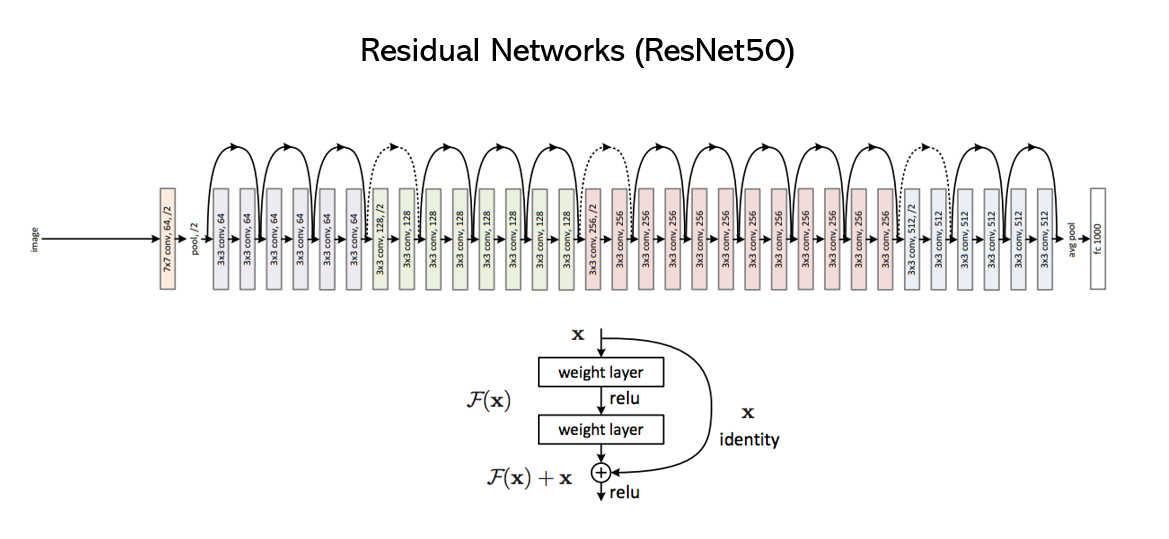
\includegraphics[width=0.8\textwidth]{./hw2/artifacts/4451f11509ee37d5155e5d429a8e4a0a.png}
        \caption{Example Image}
        \label{fig:image}
    \end{figure}
    
\end{document}